\let\negmedspace\undefined
\let\negthickspace\undefined
\documentclass[journal]{IEEEtran}
\usepackage[a5paper, margin=10mm, onecolumn]{geometry}
%\usepackage{lmodern} % Ensure lmodern is loaded for pdflatex
\usepackage{tfrupee} % Include tfrupee package

\setlength{\headheight}{1cm} % Set the height of the header box
\setlength{\headsep}{0mm}     % Set the distance between the header box and the top of the text

\usepackage{gvv-book}
\usepackage{gvv}
\usepackage{cite}
\usepackage{amsmath,amssymb,amsfonts,amsthm}
\usepackage{algorithmic}
\usepackage{graphicx}
\usepackage{textcomp}
\usepackage{xcolor}
\usepackage{txfonts}
\usepackage{listings}
\usepackage{enumitem}
\usepackage{mathtools}
\usepackage{gensymb}
\usepackage{comment}
\usepackage[breaklinks=true]{hyperref}
\usepackage{tkz-euclide} 
\usepackage{listings}
% \usepackage{gvv}                                        
\def\inputGnumericTable{}                                 
\usepackage[latin1]{inputenc}                                
\usepackage{color}                                            
\usepackage{array}                                            
\usepackage{longtable}                                       
\usepackage{calc}                                             
\usepackage{multirow}                                         
\usepackage{hhline}                                           
\usepackage{ifthen}                                           
\usepackage{lscape}
\begin{document}

\bibliographystyle{IEEEtran}
\vspace{3cm}

\title{4.2.15}
\author{EE25BTECH11012-BEERAM MADHURI}
% \maketitle
% \newpage
% \bigskip
{\let\newpage\relax\maketitle}

\renewcommand{\thefigure}{\theenumi}
\renewcommand{\thetable}{\theenumi}
\setlength{\intextsep}{10pt} % Space between text and floats


\numberwithin{equation}{enumi}
\numberwithin{figure}{enumi}
\renewcommand{\thetable}{\theenumi}


\textbf{Question}:\\
Find the direction and normal vectors of $y=2x$. \\
\textbf{Solution}:\\\\
The line can be written as:
\begin{align}
-2x + 1y = 0
\end{align}
This equation can be expressed in terms of matrices as:
\begin{align}
\vec{n}^\top \vec{x} = c\\
\vec{n}^\top = \begin{pmatrix} -2 & 1 \end{pmatrix}\\
\vec{x} = \begin{pmatrix} x \\ y \end{pmatrix}\\
c = 0
\end{align}
where $\vec{n}$ is normal vector of the given line.

The direction vector is:
\begin{align}
\vec{m} = \begin{pmatrix} 1 \\ 2 \end{pmatrix}.
\end{align}
This is true because, if the direction vector is represented as
\begin{align}
\vec{m} = \begin{pmatrix} 1 \\ m \end{pmatrix}
\end{align}
then the normal vector can be expressed as
\begin{align}
  \vec{n} = \begin{pmatrix} -m \\ 1 \end{pmatrix} \\
  \vec{n}^\top \vec{m} =0\\
   \begin{pmatrix} -2 & 1 \end{pmatrix}\begin{pmatrix} 1 \\ 2 \end{pmatrix}=0
\end{align}
Hence, normal vector $\vec{n} = \begin{pmatrix} -2 \\ 1 \end{pmatrix}$ and direction vector  $\vec{m} = \begin{pmatrix} 1 \\ 2 \end{pmatrix}$.

\begin{figure}[H]
    \centering
    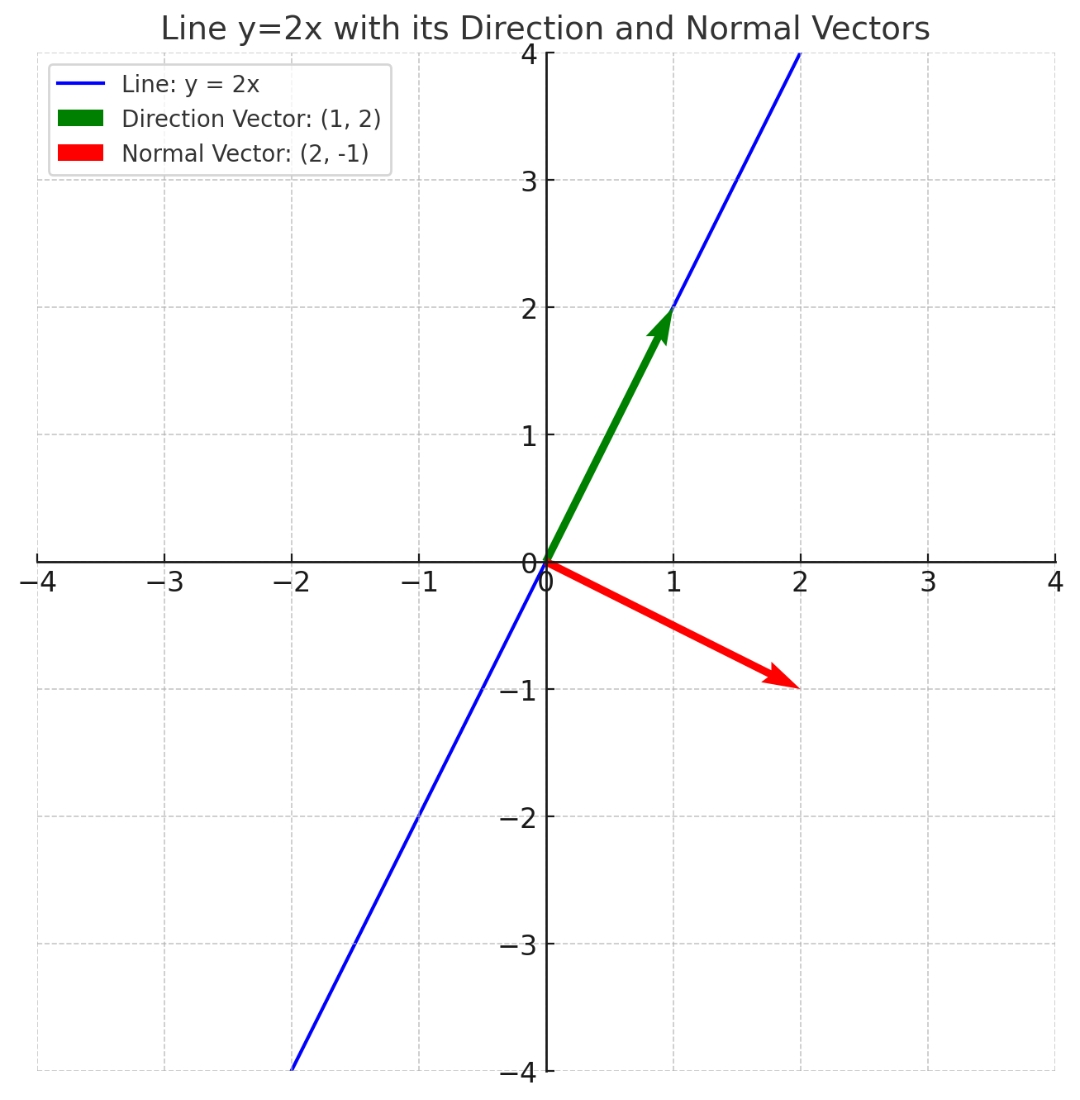
\includegraphics[width=0.75\columnwidth]{figs/graph-6.jpg}
    \caption{line y=2x}
    \label{fig:placeholder}
\end{figure}

\end{document}